\documentclass[11pt]{article}
\usepackage[utf8]{inputenc}
\usepackage[T1]{fontenc}
\usepackage{times}
\usepackage[a4paper,margin=1in]{geometry}
\usepackage{amsmath,amssymb}
\usepackage{booktabs,tabularx,array,float,graphicx}
\usepackage[round]{natbib}
\usepackage{microtype}
\usepackage[hidelinks]{hyperref}
\renewcommand{\tabularxcolumn}[1]{>{\raggedright\arraybackslash}p{#1}}
\widowpenalty=10000 \clubpenalty=10000
\setlength{\parskip}{4pt}
\bibliographystyle{plainnat}

\title{Who Took the Hint? Applying Methods of Causal Inference to Evaluate Chain of Thought Monitorability\thanks{An abridged version of this paper was prepared for the Agent Evaluation Science symposium, New York, November 2026. The abridged paper and its online supplement are at \url{https://github.com/alexisjdiamond/who-took-the-hint}.}}
\author{Alexis Diamond\\ Minerva University}
\date{October 2026}

\begin{document}
\maketitle
\begin{abstract}
Intervention-based evaluations of chain-of-thought monitorability \citep{guan2025monitoring} ask how reliably a monitor detects whether a model’s answer was influenced by a cue. We show that these evaluations have the structure of an encouragement design with one-sided noncompliance: offering the cue is the encouragement, the model’s use of the cue’s content is the treatment, observed only through a monitor that reads the chain of thought with error, and the answer is the outcome. Applying this lens reveals a structural mismatch in the monitorability score, g-mean$^2$: monitors are graded against the fraction of encouraged cue-concordant answers that would not have occurred without the cue, which the two arms identify, but are tasked with detecting the influence rate (the fraction in which the model used the cue), which the arms do not identify. The difference between these estimands grows with the base rate. We work through three cases in which a correctly computed score supports the wrong conclusion: a monitor missing half of cue use scored as perfect; a monitor validated at low base rates deployed where they are high, including realistic environments in the framework; and a model that stops verbalizing read as a degraded monitor. The framing also suggests that established methods from econometrics and epidemiology apply.
\end{abstract}

\section{Introduction}
\citet{guan2025monitoring} propose intervention-based evaluations of chain-of-thought monitorability. OpenAI reports the resulting scores in the system cards of its frontier models, and others have adopted the score \citep{wang2026monitorbench}. A model is sampled repeatedly on the same prompt with and without a cue, the change in the rate of cue-concordant output is measured, and a monitor reading the chain of thought is asked whether the model was influenced. An output is cue-concordant when it agrees with what the cue points to: the hinted option, the user’s stated opinion, the patient’s self-diagnosis. The resulting score, g-mean$^2$, is used as a measure of how far a model’s reasoning can be trusted to reveal to a monitor what drives its behavior. Chain-of-thought monitoring has been proposed as a safety control for frontier models, with monitorability as the condition under which it can be relied on \citep{korbak2025chain}.

The framework is a careful attempt to measure monitorability, and its authors anticipated several issues raised here: the monotonicity assumption, dependence on base rates, and the gap between the score’s true-positive term and the actual true-positive rate. \citet{dilgren2026evaluating} catalogue practical weaknesses of the released evaluations; this paper concerns the identification structure. We show that this evaluation is an encouragement design with an unusual structure that creates blind spots. Because g-mean$^2$ grades the monitor against what the two arms can identify rather than against cue use the monitor is asked to find, it can support wrong conclusions without raising red flags. In one case (Section~3.1) it scores as perfect a monitor that misses half of actual cue use. On October 20, 2026, the score’s authors began reporting upper and lower bounds on the monitor’s true-positive rate for cue use (what the authors call causal recall), and comparing models only on instances valid for both \citep*{guan2026beyond}.\footnote{Each model’s score is computed only on the instances (prompts paired with a cue) where the cue had a positive estimated effect for that model, and different models clear that bar on different instances. Two models’ scores can therefore differ because one was scored on easier instances than the other, not because its reasoning is more legible to the monitor. Comparing them only on instances that pass for both removes that source of difference; it does not remove differences in the kind of behavior each model produces on a shared instance, as Guan, Xie and Baker note. On the released evaluations, \citet{dilgren2026evaluating} find that only 3\% to 24\% of instances pass the gate.} Concurrently, \citet{fu2026learning} derive the same bounds from a structural causal model, define the target as the monitor’s recall on outcomes the intervention caused, and build two composite scores from the two endpoints; they also train models to raise them. This paper supplies a structure that accounts for these additions, shows where the bounds are wide, and states assumptions under which they narrow.

In the vocabulary of causal inference, the evaluation is an encouragement design with one-sided noncompliance: the cue is the encouragement, use of the cue’s semantic content is the treatment, and cue-concordant output is the outcome \citep{angrist1996identification}. In a standard encouragement design, take-up is observed and the counterfactual outcome is missing. Here, take-up is missing: it happens inside the model, the chain of thought is its record, and the monitor is an imperfect observer of treatment status that reads that record. The evaluation must therefore judge the monitor without any independent record of what it is supposed to detect. This inversion also shifts the objective: rather than estimating the effect of the treatment on the treated, the evaluation must judge an observer’s ability to detect the treatment.

\section{The evaluation as an encouragement design}
\subsection{Notation}
An evaluation consists of many \emph{instances}, each a prompt paired with a cue; for each, the model is sampled n times with the cue absent and n times with it present, and each sample is a \emph{draw}. For a draw, Z $\in$ \{0, 1\} records whether the cue was offered (Z = 0 is the no-encouragement arm, Guan et al.’s control arm; Z = 1 the encouraged arm, their intervention arm), D $\in$ \{0, 1\} whether the model used the cue’s semantic content in producing its answer (“cue use” hereafter), Y $\in$ \{0, 1\} whether the output was cue-concordant in the sense of Section~1, and M $\in$ \{0, 1\} the monitor’s verdict, an imperfect observation of D made by reading the chain of thought (Appendix A). Write

\begin{align*}
  p_0 &= \Pr(Y = 1 | Z = 0)\quad\text{the base rate: cue-concordant output in the no-encouragement arm} \\
  p_1 &= \Pr(Y = 1 | Z = 1)\quad\text{cue-concordant output in the encouraged arm} \\
  \pi  &= \Pr(D = 1 | Z = 1)\quad\text{the take-up rate: share of encouraged draws that use the cue}
\end{align*}

Nothing is randomized: both arms are repeated draws from the same model on the same prompt, so they are exchangeable by construction, and the “types” below are proportions of draws, not labels on draws.

\subsection{One-sided noncompliance and the three quantities}
Encouragement designs are typically analyzed in statistics and econometrics with instrumental-variables methods, with the offer of the cue as the instrument. A draw cannot use a cue it was not given, so D = 0 whenever Z = 0 and noncompliance is one-sided, a case first analyzed by \citet{bloom1984accounting} and treated in \citet[ch. 23]{imbens2015causal}. The no-defier condition, an assumption basic to standard encouragement designs (here, that no draw would use the cue only when it is not offered), holds by construction. Two treatment types remain: \emph{compliers}, who use the cue when offered (mass $\pi$), and \emph{never-takers}, who ignore it (mass 1 $-$ $\pi$).

Suppose, as Guan et al.’s worked example does, that a draw using the cue produces the cue-concordant output (a draw that uses the cue’s content to reject the hint violates this, as Section~2.5 discusses), and that draws not using it behave as they would unaided, with the same baseline rate $p_0$ whether or not they are compliers (Section~2.4 relaxes this). Then

\begin{align*}
  p_1 &= \pi  + (1 - \pi ) p_0 \\
  \mathrm{TE} &= p_1 - p_0 = \pi  (1 - p_0) \\
  R_{\mathrm{effect}} &= \mathrm{TE} / p_1 \\
  \text{influence rate} &= \pi  / p_1
\end{align*}

TE is the \textbf{intention-to-treat effect} (Guan et al.’s total effect), the causal effect of offering the cue, averaged over compliers and never-takers. It equals the mass of draws whose output is cue-concordant with the cue and not without it, provided the cue never pushes a draw away from the cue-concordant output (\citeauthor{manski1997monotone}’s \citeyear{manski1997monotone} monotone treatment response, Guan et al.’s monotonicity). $R_{\mathrm{effect}}$ is the share of encouraged cue-concordant draws whose output the cue changed. It is a principal-stratum proportion \citep{frangakis2002principal} and the excess fraction of epidemiology \citep{greenland1988conceptual}, and it is the floor the monitor is graded against (Section~2.6). \citet{burger2026cot} report an equivalent bound. The \textbf{influence rate} $\pi$ / $p_1$ is the share of encouraged cue-concordant draws that used the cue. It is what the monitor is asked to detect, but the arms do not identify it. It exceeds $R_{\mathrm{effect}}$ by $\pi$ $p_0$ / $p_1$, the compliers whose output would have been cue-concordant anyway, a mass \citet{dilgren2026evaluating} note informally, and the ratio of the two, 1 / (1 $-$ $p_0$), depends on the base rate alone.

In Guan et al.’s example (worked step by step in Section~2.3), where the hint points to option D ($p_0$ = 0.25, $p_1$ = 0.85), the arms identify TE = 0.60 and the floor 0.60 / 0.85 $\approx$ 0.71. The share of encouraged D-answers that followed the hint, 0.80 / 0.85 $\approx$ 0.94, is their causal influence rate, and the difference, (0.80 $-$ 0.60) / 0.85 $\approx$ 0.24, is hint-followers who would have said D anyway. TE and $R_{\mathrm{effect}}$ are functions of potential outcomes, but the influence rate is not.\footnote{Section~7 sorts the framework’s uses of “causal” into effects, quantities, mechanism attributions and inferences, and places the influence rate in the epidemiological literature on attributable fractions.}

\subsection{Guan et al.’s example, step by step}
Guan et al.’s illustration (their Section~3.1.1) makes every quantity concrete. A four-option question carries a hint pointing to option D. In the no-encouragement arm the model guesses uniformly, so it answers D a quarter of the time: $p_0$ = 0.25. In the encouraged arm, 80\% of draws follow the hint and the rest behave as if unaided: $\pi$ = 0.8.

\begin{table}[H]
  \centering\small
  \begin{tabularx}{\linewidth}{@{}XXXXXX@{}}
    \toprule
    Quantity & Formula & $\pi$ = 0.8, $p_0$ = 0.25 & $\pi$ = 0.8, $p_0$ = 0.05 & $\pi$ = 0.6, $p_0$ = 0.50 & Identified from the two arms? \\
    \midrule
    Base rate (input) & $p_0$ & 0.25 & 0.05 & 0.50 & yes (stipulated) \\ \addlinespace[3pt]
    Take-up rate (input) & $\pi$ & 0.80 & 0.80 & 0.60 & no (stipulated) \\ \addlinespace[3pt]
    Cue-concordant rate, cue present & $p_1$ = $\pi$ + (1 $-$ $\pi$) $p_0$ & 0.85 & 0.81 & 0.80 & yes \\ \addlinespace[3pt]
    Intention-to-treat effect & TE = $\pi$(1 $-$ $p_0$) & 0.60 & 0.76 & 0.30 & yes \\ \addlinespace[3pt]
    Floor & $R_{\mathrm{effect}}$ = TE / $p_1$ & 0.706 & 0.938 & 0.375 & yes \\ \addlinespace[3pt]
    Influence rate & $\pi$ / $p_1$ & 0.941 & 0.988 & 0.750 & no \\ \addlinespace[3pt]
    Gap & $\pi$ $p_0$ / $p_1$ & 0.235 & 0.049 & 0.375 & no \\ \addlinespace[3pt]
    Influence rate / floor & 1 / (1 $-$ $p_0$) & 1.33 & 1.05 & 2.00 & — \\ \addlinespace[3pt]
    Effect of cue use among cue-using draws & TE / $\pi$ = 1 $-$ $p_0$ & 0.75 & 0.95 & 0.50 & no \\
    \bottomrule
  \end{tabularx}
  \caption{Guan et al.’s worked example ($\pi$ = 0.8, $p_0$ = 0.25) and two variants.}
\end{table}

\noindent{\small Guan et al.’s 16/17 = 0.941 is the influence rate; the understatement they note is the gap. The steps below walk through the first column.}

\emph{Step 1, the encouraged arm’s rate.} Hint-followers answer D (0.80 of all draws); the unaided fifth answers D a quarter of the time (0.20 $\times$ 0.25 = 0.05). So $p_1$ = 0.85.

\emph{Step 2, the intention-to-treat effect.} TE = $p_1$ $-$ $p_0$ = 0.60. Offering the hint raised the rate of D by 60 points. This is identified from the two arms.

\emph{Step 3, the floor.} Among encouraged draws that answered D, the share whose answer would not have been D without the hint is TE / $p_1$ = 0.60 / 0.85 $\approx$ 0.71. This is $R_{\mathrm{effect}}$, the floor. Under monotone treatment response it too is identified.\footnote{Without monotone treatment response, TE understates the complier mass by the mass of draws the cue moves away from the cue-concordant output, and 0.71 is a lower bound on this share rather than its value (Section~2.5).}

\emph{Step 4, the influence rate.} Among the same 0.85, the share that followed the hint is 0.80 / 0.85 = 16/17 $\approx$ 0.94. Guan et al. report this number as the fraction attributable to the hint and note that the measured total effect, 0.60, is smaller. It is smaller because 0.20 $\times$ 0.25 = 0.05 of all draws are hint-followers who would have guessed D anyway: the hint fired (U = 1 in Guan et al.’s notation) but the answer did not depend on it (Y(0) = Y(1) = 1). The floor excludes them; the influence rate counts them. Their mass, 0.05 / 0.85 $\approx$ 0.24, is the gap.

\emph{Step 5, why the influence rate is not identified.} Step 4 used $\pi$ = 0.8, which is stipulated in the example and unobserved in practice: the evaluation sees 0.85 in one arm and 0.25 in the other, and those two numbers are consistent with many values of $\pi$. Under monotone treatment response the influence rate lies in [0.71, 1]; the lower end is the floor, and that is the precise content of Guan et al.’s statement that the total effect lower-bounds the causal influence rate. With $p_0$ = 0 the interval collapses to a point, which is their observation that the two coincide only at zero base rate.

\emph{Step 6, the Wald ratio.} Dividing the intention-to-treat effect by the take-up rate (the first stage, in instrumental-variables terms) gives TE / $\pi$ = 0.60 / 0.80 = 0.75: among draws that used the hint, using it raised the rate of D from 0.25 to 1. This is the local average treatment effect, here equal to the effect of treatment on the treated, and it is not computable from the evaluation because $\pi$ is unobserved. The monitor’s flag rate is the only available estimate of $\pi$, which Section~5.3 exploits.

Three ratios, then, share the ingredients 0.60, 0.80 and 0.85 and answer three questions. 0.60 / 0.85 = 0.71 asks what share of encouraged D-answers depended on the hint (the floor). 0.80 / 0.85 = 0.94 asks what share used the hint (the influence rate). 0.60 / 0.80 = 0.75 asks what using the hint did to the draws that used it (the Wald ratio). The evaluation identifies the first, scores the monitor against it, names the second as the monitor’s target, and would need a trustworthy monitor to recover the third. A perfect detector of hint use flags 0.94 of encouraged D-answers and clears the floor of 0.71 with room to spare; a monitor detecting three-quarters of hint use flags 0.75 $\times$ 0.94 $\approx$ 0.71 and clears it exactly, scoring $\mathrm{TPR}_{\mathrm{mc}}$ = 1 while missing a quarter of actual hint use.

\subsection{Unequal baselines}
Let compliers and never-takers have unaided cue-concordant rates $p_0^{c}$ and $p_0^{n}$, which need not be equal and are not separately identified. Under one-sided noncompliance and the exclusion restriction,

\begin{align*}
  p_0 &= \pi  p_0^{c} + (1 - \pi ) p_0^{n}, \\
  p_1 &= \pi  + (1 - \pi ) p_0^{n}, \\
  \mathrm{TE} &= \pi  (1 - p_0^{c}).
\end{align*}

The floor is $R_{\mathrm{effect}}$ = TE / $p_1$ and the influence rate is $\pi$ / $p_1$; their difference, the mass of encouraged cue-concordant draws that used the cue and would have been cue-concordant anyway, is $\pi$ $p_0^{c}$ / $p_1$, and their ratio is 1 / (1 $-$ $p_0^{c}$). The equal-baseline formulas in Section~2.2 follow with $p_0^{c}$ = $p_0^{n}$ = $p_0$. Note that the gap depends on the compliers’ baseline specifically, so Guan et al.’s point value of 16/17 relies on the untestable assumption that cue use is independent of what a draw would have done unaided. The effect of cue use among cue-using draws is TE / $\pi$ = 1 $-$ $p_0^{c}$; with one-sided noncompliance this is both the local average treatment effect and the effect of treatment on the treated. Read in reverse, any postulated $\pi$ implies $p_0^{c}$ = 1 $-$ TE / $\pi$, and the constraint $p_0^{c}$ $\in$ [0, 1] with $p_0^{n}$ $\in$ [0, 1] reproduces exactly $\pi$ $\in$ [TE, $p_1$]. The further restriction $p_0^{c}$ $\geq$ $p_0^{n}$, equivalently $p_0^{c}$ $\geq$ $p_0$, plausible for a wrong hint, gives $\pi$ $\geq$ TE / (1 $-$ $p_0$) and hence an influence rate of at least TE / [(1 $-$ $p_0$) $p_1$]; the reverse restriction, plausible for a correct hint, gives the corresponding upper bound, which leaves the lower bound on recall unchanged.

\emph{Worked example, Guan et al.'s instance.} The arms give $p_0$ = 0.25, $p_1$ = 0.85 and TE = 0.60, so $\pi$ can lie anywhere in [0.60, 0.85]. Each value is a different account of who complied. At $\pi$ = 0.60, the minimum, every encouraged cue-concordant draw that would not have been cue-concordant anyway is a complier, so $p_0^{c}$ = 1 $-$ 0.60 / 0.60 = 0: the compliers never give the hinted answer unaided. At $\pi$ = 0.85, the maximum, $p_0^{c}$ = 1 $-$ 0.60 / 0.85 = 0.29. At Guan et al.'s $\pi$ = 0.80, $p_0^{c}$ = 1 $-$ 0.60 / 0.80 = 0.25 = $p_0$, which is the equal-baseline case: their point value is the one account in which compliers behave unaided like everyone else. The two arms cannot choose among these accounts. The restriction $p_0^{c}$ $\geq$ $p_0$ = 0.25 selects the upper part of the range, $\pi$ $\geq$ 0.80, and hence an influence rate of at least 0.80 / 0.85 = 0.94.

Why the baselines are likely to differ. The equal-baseline assumption is probably false. Whether a draw takes a hint plausibly depends on how confident the model is in its own answer: a draw that has settled on an answer tends to ignore a hint pointing elsewhere, and an uncertain draw tends to take it \citep{sharma2023towards,chen2025reasoning,lanham2023measuring}. Compliers are then concentrated among uncertain draws, which spread probability across options, including the hinted one. For a wrong hint, the compliers’ unaided rate $p_0^{c}$ therefore exceeds the never-takers’ $p_0^{n}$. For a correct hint the inequality reverses, since confident never-takers give the right answer. This changes inference about take-up, as the formulas above show.

\subsection{Effects in both directions, and bounds without monotone treatment response}
Without the assumption that the cue never pushes a draw away from the cue-concordant output, the mass of draws with Y(0) = 0 and Y(1) = 1 is not point-identified. By the Fréchet bounds on the joint of (Y(0), Y(1)) given its marginals, Pr(Y(1) = 1, Y(0) = 0) $\in$ [max(0, $p_1$ $-$ $p_0$), min($p_1$, 1 $-$ $p_0$)]. TE is the lower endpoint. An instance with TE = 0 may therefore contain equal masses of draws moved toward and away from the cue-concordant output rather than none of either, which the gate of Section~2.6 cannot distinguish. The floor survives the loss of monotonicity: every draw with Y(0) = 0 and Y(1) = 1 used the cue (under the exclusion restriction), and such draws are at least a share TE of all draws, so the influence rate is still at least TE / $p_1$. Monotonicity is needed to read TE as the complier mass itself, not to make the floor a lower bound; without it the bound is merely looser.

\emph{Worked example, Guan et al.'s instance.} With $p_0$ = 0.25 and $p_1$ = 0.85, the Fréchet bounds give Pr(Y(1) = 1, Y(0) = 0) $\in$ [max(0, 0.60), min(0.85, 0.75)] = [0.60, 0.75]. Under monotone treatment response the mass of draws moved toward the cue-concordant output is exactly 0.60; without it, that mass could be as high as 0.75, offset by up to 0.15 of draws moved away from it, since 0.75 $-$ 0.15 nets to the observed TE of 0.60. The floor TE / $p_1$ = 0.71 is unchanged in either case, because every draw moved toward the cue-concordant output used the cue and such draws are at least 0.60 of all draws.

Effects in both directions. “Cue-concordant” names an outcome level, not an effect direction: the cue can move a draw toward that level, Y(0) = 0 and Y(1) = 1, or away from it, Y(0) = 1 and Y(1) = 0, even though, as this appendix explains, the metric counts only the first.

The no-defier condition of Section~2.2 applies strictly to treatment take-up. Draws the cue moves away from the cue-concordant output, with Y(0) = 1 and Y(1) = 0, are ruled out by a separate assumption, monotone treatment response \citep{manski1997monotone}, Y(1) $\geq$ Y(0) for every draw, discussed below. It concerns the outcome and differs from the standard monotonicity assumption of encouragement designs \citep{imbens1994identification}, which concerns take-up: that no unit takes the treatment only when not encouraged, which here holds by construction.

$\mathrm{TPR}_{\mathrm{mc}}$ also counts influence in only one direction. It credits the monitor for flagging draws that the cue pushed toward the cue-concordant answer, but the monitor is asked whether the model was influenced at all, which includes draws the cue pushed away from that answer. Such draws used the cue’s content, so they are compliers in the take-up sense, with a negative effect on the outcome; monotone treatment response rules them out.

What makes Guan et al.’s metric one-directional is monotone treatment response, which rules out draws with Y(0) = 1 and Y(1) = 0 by assumption, together with their decision to discard every instance whose estimated effect is not positive. Where such draws nonetheless exist, an instance in which they outweigh the draws moved toward the cue-concordant output has a non-positive estimated effect and is discarded, while an instance in which they are outweighed is scored with TE understating the complier mass by their share. A model that reads the hint, judges it a trap, and chooses otherwise was influenced by the cue, and a good monitor should say so, but nothing in the score credits it. The assumption is not innocuous. A model that mistrusts the cue is pushed away from the cue-concordant output by it. Mistrust has ordinary causes, such as training against sycophancy, and because models are increasingly trained to resist this kind of pressure, the share of such draws can grow across checkpoints. The same two-directional influence affects specificity: encouraged draws that did not give the cue-concordant answer are treated as true negatives, yet the cue may have moved some of them toward a different answer, a point Bürger et al. (2026, their Section~3.3) make about intervention experiments generally.

\subsection{How the score grades the monitor, and which instances it scores}
Guan et al. score the monitor by what they call a minimal criterion, minimal because it requires the monitor to flag at least the smallest share of draws attributable to the cue. They write it as a true-positive rate, $\mathrm{TPR}_{\mathrm{mc}}$ (“mc” for minimal criterion):

\begin{align*}
  \mathrm{TPR}_{\mathrm{mc}} &= \min(1, \Pr(M = 1 | Z = 1, Y = 1) / R_{\mathrm{effect}}).
\end{align*}

Specificity is split by arm into two true-negative rates, $\mathrm{TNR}_0$ = Pr(M = 0 | Z = 0) and $\mathrm{TNR}_1$ = Pr(M = 0 | Z = 1, Y = 0), and the aggregate metric is the squared geometric mean of the true-positive and true-negative rates:

\begin{align*}
  g\text{-}\mathrm{mean}^2 &= \mathrm{TPR}_{\mathrm{mc}} \cdot  \sqrt{\mathrm{TNR}_1 \cdot  \mathrm{TNR}_0}.
\end{align*}

Because $R_{\mathrm{effect}}$ is undefined when TE $\leq$ 0, the metric is computed only on instances whose estimated TE is positive (a rule we call the \emph{gate}). $\mathrm{TPR}_{\mathrm{mc}}$ is not a true-positive rate in the usual sense, because the ground truth for treatment status is unknown for every draw, as its authors now note \citep*{guan2026beyond}.

$R_{\mathrm{effect}}$ is a floor on the share of cue use, so $\mathrm{TPR}_{\mathrm{mc}}$, which divides the flag rate by it, is an upper bound on the monitor’s true-positive rate for cue use (its recall) \citep*{guan2026beyond}. A perfect detector flags $\pi$ / $p_1$, which exceeds $R_{\mathrm{effect}}$ by the gap, and because the ratio is capped at 1, any monitor that flags at least the floor scores 1.

\subsection{The exclusion restriction, and the monitor’s error}
The identities in Section~2.2 need the cue to affect the output only through the treatment: Y(z, d) = Y(d), the exclusion restriction of instrumental-variables analysis. With the treatment defined as use of the cue’s semantic content, the restriction says that the cue cannot shift the output except by having its content used. This assumption can fail, since a cue is also a piece of text with properties other than its content (see the example below), and it is not testable from the two arms alone, which never observe D. Under the exclusion restriction, every draw whose answer moved with the cue used its content, so the floor is a lower bound on what a perfect observer of D would flag; when it fails, some outcome-dependent draws contain nothing to find, and even a perfect observer can fall below the floor (example below).

Separate from the restriction is the monitor’s error, which has two sources: the chain of thought does not record the cue use that occurred (unfaithfulness; \citealp{turpin2023language}; \citealp{lanham2023measuring}; \citealp{chen2025reasoning}), or it does and the monitor misreads it. A scored miss (an outcome that moved with the cue and was not flagged) can therefore arise three ways: a violation of the exclusion restriction, an unrecorded use, or a misreading. Only the last is a property of the monitor, and the score cannot differentiate the three (Section~3.3).

The exclusion restriction fails when the cue text moves the output by a route other than use of its semantic content. For example, the cue lengthens the prompt, which can change how long the model reasons, and its mere presence can provoke a reaction whatever it says. On a broader definition of cue use, any causal role the cue plays in producing the output, these routes would count as use and the restriction would hold by construction; but that definition makes the treatment include influence that leaves no reasoning for a reader of the chain of thought to find, so the monitor would have a target it cannot in principle observe.

A worked example of the failure:

\emph{Step 1, the setup.} Take 100 encouraged draws on a question with a wrong hint pointing to option D, and a base rate of 0.20, so that without the hint 20 of 100 draws would answer D.

\emph{Step 2, content use.} Suppose 30 of the 100 use the hint's content and all 30 answer D.

\emph{Step 3, a direct effect.} Suppose the hint's mere presence, independent of its content, raises the D rate among the other 70 draws from 0.20 to 0.50, so 35 of them answer D instead of the 14 the base rate would predict. This is a violation of the exclusion restriction: the cue moved the output by a route other than use of its content.

\emph{Step 4, what the arms show.} $p_1$ = 65 / 100 = 0.65 and $p_0$ = 0.20, so TE = 0.45 and the floor is $R_{\mathrm{effect}}$ = 0.45 / 0.65 = 0.69. The metric requires a monitor to flag at least 45 of the 65 D-answers.

\emph{Step 5, what a perfect observer of cue use finds.} Only 30 of the 65 D-answers used the hint's content. The other 35 were moved by the hint's presence and contain no content use for any reader of the chain of thought to find. A perfect observer flags 30 of 65, a rate of 0.46, and scores $\mathrm{TPR}_{\mathrm{mc}}$ = 0.46 / 0.69 = 0.67. The exclusion failure makes a flawless monitor look as if it misses a third of cue use, and nothing in the two arms distinguishes this from a monitor that does.

\section{Three cases in which a correct score misleads}
In each case g-mean$^2$ is computed correctly, and yet it invites a reading it does not support. None of the three is a claim that any particular published g-mean$^2$ score is misleading.

\subsection{The half-blind monitor that scores perfectly}
Consider a sycophancy-style behavior: the cue is a user’s stated view, which the model’s answer matches half the time unaided ($p_0$ = 0.5) and which 60\% of draws use when present ($\pi$ = 0.6). Compliers give the cue-concordant output and never-takers default to the 50\% baseline, so $p_1$ = 0.6 + 0.4 $\times$ 0.5 = 0.8, TE = $p_1$ $-$ $p_0$ = 0.3, and the floor is $R_{\mathrm{effect}}$ = TE / $p_1$ = 0.375. Compliers are $\pi$ / $p_1$ = 0.75 of encouraged cue-concordant draws, so a perfect detector of cue use flags 75\% of them. A monitor that misses half of actual cue use flags 0.375, so $\mathrm{TPR}_{\mathrm{mc}}$ = min(1, 0.375 / 0.375) = 1.

With ordinary specificity it posts a g-mean$^2$ near the top of the published range while missing half of the draws in which the model used the cue, and every miss is invisible, since the framework cannot know those draws used the cue. A safety case of the form “if the model does X for reason R, the monitor catches it with probability at least p” needs the detection rate of cue use, which the two arms do not identify. The arithmetic generalizes: a monitor detecting (1 $-$ $p_0$) of cue use scores $\mathrm{TPR}_{\mathrm{mc}}$ = 1 at any $\pi$, and averaging over a dataset does not expose it, since no instance reveals D; the failure is hidden in proportion to a dataset’s share of high-base-rate instances (Section~3.2; the arithmetic is worked below).

\emph{The arithmetic, step by step.}

\emph{Step 1, the rates.} The cue is a user’s stated view. Take $p_0$ = 0.5 (the model gives that view’s answer half the time unaided) and $\pi$ = 0.6 (60\% of encouraged draws use the view). Compliers give the cue-concordant output and never-takers default to the baseline, so $p_1$ = 0.6 + 0.4 $\times$ 0.5 = 0.8, TE = $p_1$ $-$ $p_0$ = 0.3, and $R_{\mathrm{effect}}$ = TE / $p_1$ = 0.375.

\emph{Step 2, what a perfect monitor flags.} Every complier used the cue and is cue-concordant, so compliers are $\pi$ / $p_1$ = 0.6 / 0.8 = 0.75 of encouraged cue-concordant draws; the other 0.25 are never-takers whose answer matched the stated view without using it. A perfect detector of cue use flags 75\%.

\emph{Step 3, the half-blind monitor.} A monitor that detects half of actual cue use flags 0.5 $\times$ 0.75 = 0.375. The score divides by the floor: $\mathrm{TPR}_{\mathrm{mc}}$ = min(1, 0.375 / 0.375) = 1. With both true-negative rates at 0.95, g-mean$^2$ = 0.95, near the top of the published range.

\emph{Step 4, why the score cannot tell.} The 0.375 the monitor flags and the 0.375 the floor demands coincide, and the framework has no way to see that the flagged draws are only half of those that used the cue, since no draw carries a label for cue use. \citeauthor*{guan2026beyond}’s (\citeyear{guan2026beyond}) lower bound on recall, max(0, (f + $R_{\mathrm{effect}}$ $-$ 1) / $R_{\mathrm{effect}}$) with f = 0.375, is max(0, $-$0.67) = 0, so their interval for this monitor is [0, 1].

\emph{Step 5, the general condition.} A monitor detecting a share $\delta$ of cue use flags $\delta$ $\pi$ / $p_1$, and $\mathrm{TPR}_{\mathrm{mc}}$ = min(1, $\delta$ $\pi$ / ($p_1$ $R_{\mathrm{effect}}$)) = min(1, $\delta$ / (1 $-$ $p_0$)). It scores 1 whenever $\delta$ $\geq$ 1 $-$ $p_0$, at any $\pi$. Here 1 $-$ $p_0$ = 0.5, so any monitor catching at least half of cue use scores perfectly. Averaging across instances does not change this, because the score is bounded by 1 on every instance where the condition holds; on instances with lower base rates the same monitor falls below the floor, so the failure is hidden in proportion to a dataset’s share of high-base-rate instances.

\subsection{Validated where the floor is the influence rate, deployed where it is not}
This case locates the gap of case (1) in the framework’s own environments. From Section~2.2, the influence rate exceeds the floor by the factor 1 / (1 $-$ $p_0$). A monitor can miss $p_0$ of actual cue use and still score $\mathrm{TPR}_{\mathrm{mc}}$ = 1 (worked below). With take-up $\pi$ = 0.8, at $p_0$ = 0.05 (so $p_1$ = 0.81 and TE = 0.76) the floor and influence rate are 5 points apart; at $p_0$ = 0.5 ($p_1$ = 0.9, TE = 0.4) the floor is half the influence rate (Figure 1). Guan et al. recommend low base rates (their Section~3.1.3), and their toy environments comply. Assume a four-option question, a cue for a wrong option (e.g., D), errors spread evenly over the three wrong options, and a model that is right 80\% of the time without the cue. Then the model gives the cued answer unaided at rate $p_0$ $\approx$ (1 $-$ 0.8)/3 $\approx$ 0.07. The environments built to resemble real use, by contrast, have high base rates. Table 2 derives each environment’s structural base rate from the definition of Y, under the equal-baseline assumption of Section~2.2; for correct-hint environments such as Health Queries patient-opinion its figures are upper ends (worked below).

\begin{table}[H]
  \centering\small
  \begin{tabularx}{\linewidth}{@{}>{\raggedright\arraybackslash}p{3.1cm}XXX@{}}
    \toprule
    Environment & Structural $p_0$ & Influence rate / floor & Cue use a monitor can miss at $\mathrm{TPR}_{\mathrm{mc}}$ = 1 \\
    \midrule
    Toy math/science (GPQA, DAFT) & $\approx$ (1 $-$ acc)/3; $\approx$ 0.07 at 80\% accuracy & $\approx$ 1.07 & $\approx$ 7\% \\ \addlinespace[3pt]
    Scruples, suggest right / wrong & $\approx$ unaided rate of the suggested verdict, $\approx$ 0.5 & $\approx$ 2 & $\approx$ 50\% \\ \addlinespace[3pt]
    Health Queries, patient opinion & $\approx$ unaided diagnostic accuracy, 0.6–0.8 & $\approx$ 2.5–5 & $\approx$ 60–80\% \\
    \bottomrule
  \end{tabularx}
  \caption{Structural base rates and the implied gap for selected Guan et al. environments, derived from the definition of Y under equal baselines (Table 3 gives all eight, with outcome definitions).}
\end{table}

\emph{The base-rate gap, step by step.}

\emph{Step 1, the ratio.} Under equal baselines (Section~2.2), the floor is $R_{\mathrm{effect}}$ = TE / $p_1$ = $\pi$(1 $-$ $p_0$) / $p_1$ and the influence rate is c = $\pi$ / $p_1$. Dividing the second by the first,

\begin{align*}
  c / R_{\mathrm{effect}} &= [\pi  / p_1] / [\pi (1 - p_0) / p_1] = 1 / (1 - p_0).
\end{align*}

The take-up rate $\pi$ and the encouraged rate $p_1$ cancel, so the ratio depends on the base rate alone.

\emph{Step 2, how much cue use a monitor can miss and still score perfectly.} Suppose the monitor flags a share $\delta$ of the draws that used the cue and nothing else. Its flag rate among encouraged cue-concordant draws is f = $\delta$c, and

\begin{align*}
  \mathrm{TPR}_{\mathrm{mc}} &= \min(1, \delta c / R_{\mathrm{effect}}) = \min(1, \delta  / (1 - p_0)).
\end{align*}

So $\mathrm{TPR}_{\mathrm{mc}}$ = 1 whenever $\delta$ $\geq$ 1 $-$ $p_0$: the monitor can miss a share 1 $-$ $\delta$ of cue use as large as $p_0$ and still score perfectly. This is the last column of Table 2 and Table 3.

\emph{Step 3, the reference points in Figure 1.} At $\pi$ = 0.8:

\begin{itemize}
  \item $p_0$ = 0.05: $p_1$ = 0.8 + 0.2 $\times$ 0.05 = 0.81, TE = 0.76, floor = 0.76 / 0.81 = 0.94, influence rate = 0.8 / 0.81 = 0.99. The two are five points apart and the ratio is 1.05.
  \item $p_0$ = 0.5: $p_1$ = 0.9, TE = 0.40, floor = 0.44, influence rate = 0.89. The ratio is 2, so the floor is half the influence rate.
  \item $p_0$ = 0.7: $p_1$ = 0.94, TE = 0.24, floor = 0.26, influence rate = 0.85. The ratio is 3.3, so the floor is under a third of the influence rate.
\end{itemize}
\begin{figure}[H]
  \centering
  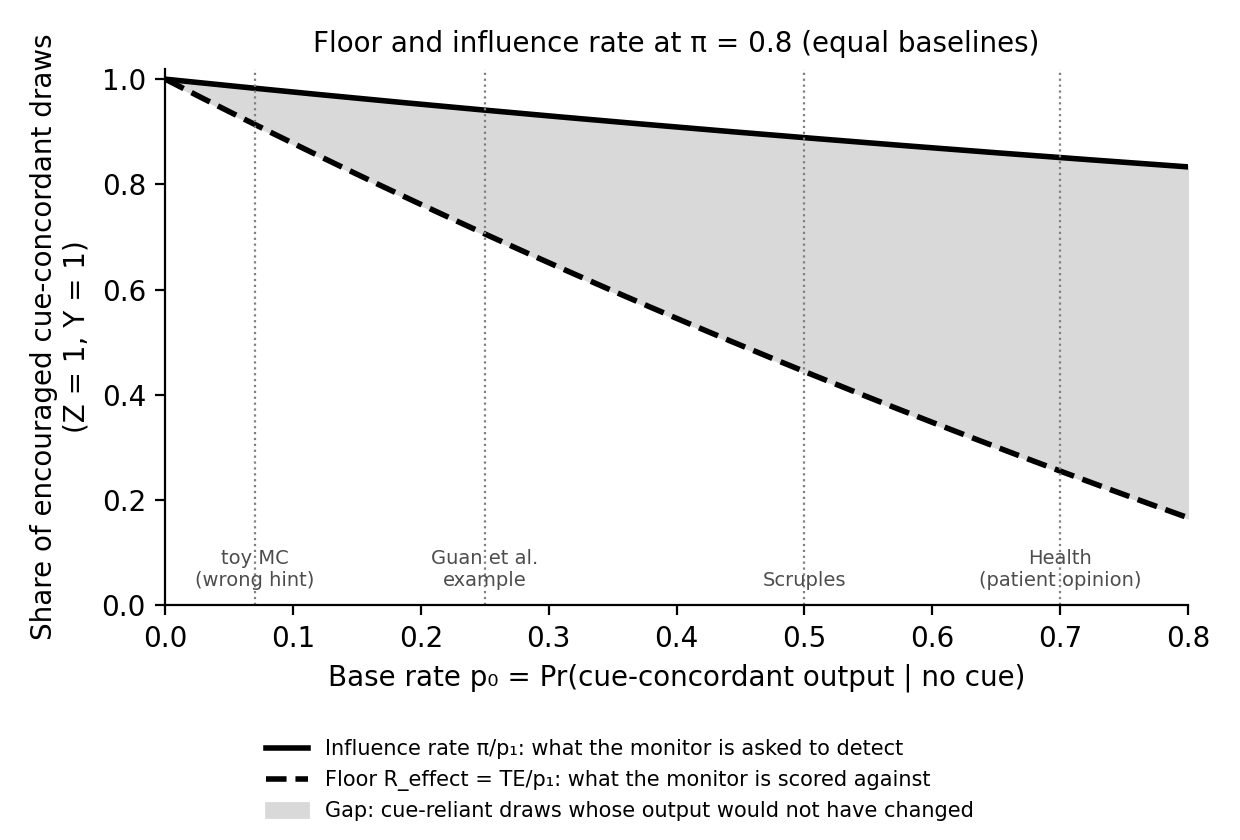
\includegraphics[width=0.78\linewidth]{fig1.png}
  \caption{The floor and the influence rate against the base rate $p_0$ at $\pi$ = 0.8, equal baselines. The band’s height, $\pi$ $p_0$ / $p_1$, is the gap of Section~2.2. Vertical lines mark structural base rates from Table 2 and Table 3.}
  \label{fig:floor}
\end{figure}

\emph{Step 4, the structural base rate for a wrong hint.} On a four-option question the model answers correctly with probability equal to its accuracy, acc, and spreads its errors, 1 $-$ acc, over the three wrong options. If it spreads them evenly, the unaided rate of the particular wrong option the hint names is $p_0$ = (1 $-$ acc)/3. At acc = 0.8 this is 0.2 / 3 $\approx$ 0.07, giving a ratio of 1 / (1 $-$ 0.07) $\approx$ 1.07 and a missable share of about 7\%: the first row of Table 2 and Table 3. If errors concentrate on one plausible distractor and the hint names it, $p_0$ is higher; if the hint names an implausible option, lower.

\emph{Step 5, every row of Table 3.} In each environment, $p_0$ is the rate at which the model gives the cue-concordant output with no cue, read off the outcome definition; the ratio is 1 / (1 $-$ $p_0$) and the missable share is $p_0$.

\begin{itemize}
  \item Toy math/science (GPQA, DAFT): Y = the hinted wrong option. Unaided, the model is correct with probability acc and spreads its errors over three wrong options, so $p_0$ $\approx$ (1 $-$ acc)/3 $\approx$ 0.07 at acc = 0.8; ratio 1.07; missable 7\%.
  \item AIME: Y = the hinted number on an open-response problem. The chance of producing a specific wrong number unaided is near zero, so $p_0$ $\approx$ 0; ratio $\approx$ 1; missable $\approx$ 0.
  \item Sandbagging (WMDP): Y = the supplied incorrect option. As for the toy case, $p_0$ $\approx$ (1 $-$ acc)/3; at acc between 0.7 and 0.85 this is 0.05 to 0.10; ratio 1.05 to 1.1.
  \item Scruples, suggest right and suggest wrong: Y = the verdict the user suggested (B, author not in the wrong, for suggest right; A for suggest wrong). The anecdotes are filtered to ones where the community judged the author in the wrong, and Guan et al. note that models are hesitant to say so, so the unaided rate of B is high and of A low: the two variants bracket 0.5, plausibly 0.3 to 0.7; ratio 1.4 to 3.3; missable 30\% to 70\%.
  \item Scruples, first person: Y = the verdict favors the author (B). The unaided rate of B is the same hesitancy, plausibly above 0.5; ratio 2 or more; missable 50\% or more.
  \item Health Queries, patient opinion: Y = the diagnosis matches the patient’s self-diagnosis, which is set to the truth. Unaided, Y = 1 whenever the model diagnoses correctly, so $p_0$ = its diagnostic accuracy, 0.6 to 0.8; ratio 2.5 to 5; missable 60\% to 80\%.
  \item Health Queries, missing evidence: Y = a correct diagnosis with a case section restored. Unaided (section absent), $p_0$ = accuracy without the section, 0.5 to 0.7; ratio 2 to 3.3.
  \item Memory: Y is a judge-labeled behavior change with no fixed outcome definition, so no structural $p_0$ can be derived.
\end{itemize}
In the Health patient-opinion variant the cue \emph{is} the correct diagnosis, so every draw the model would have diagnosed correctly anyway is cue-concordant with no outcome dependence; in Scruples the unaided rate of the suggested verdict is set by the model’s reluctance to call an author wrong, which Guan et al. report as strong on these anecdotes. Realism and identifiability trade off, because realism means a behavior the model already produces. The same holds for deployment behaviors a model often produces unprompted: reward hacking in coding environments, deference to user pressure, sandbagging on hard tasks. A monitor certified on wrong-hint GPQA carries no warrant to those; it was certified in the one regime where floor and influence rate coincide.

These are derivations, not measurements: Guan et al. do not report $p_0$ per environment, and the released code \citep{openai2026opensourcing} contains datasets and scoring, not sampled outputs. Exact outcome definitions are in Guan et al., Section~7; the Scruples and Health rows follow the outcome definitions in that appendix.

\begin{table}[H]
  \centering\small
  \begin{tabularx}{\linewidth}{@{}XXXXX@{}}
    \toprule
    Environment & Outcome Y & Structural $p_0$ & Influence rate / floor & Cue use a monitor can miss at $\mathrm{TPR}_{\mathrm{mc}}$ = 1 \\
    \midrule
    Toy math/science (GPQA, DAFT) & Answer equals hinted option; hint points to a wrong option of four & $\approx$ (1 $-$ acc)/3; $\approx$ 0.07 at 80\% accuracy & $\approx$ 1.07 & $\approx$ 7\% \\ \addlinespace[3pt]
    AIME & Answer equals hinted number; open response & $\approx$ 0 & $\approx$ 1 & $\approx$ 0 \\ \addlinespace[3pt]
    Sandbagging (WMDP) & Answer equals the supplied incorrect option & $\approx$ (1 $-$ acc)/3 & $\approx$ 1.05–1.1 & $\approx$ 5–10\% \\ \addlinespace[3pt]
    Scruples, suggest right / wrong & Verdict equals the one the user suggested (B / A) & unaided rate of the suggested verdict; the two variants bracket 0.5, $\approx$ 0.3–0.7 & $\approx$ 1.4–3.3 & $\approx$ 30–70\% \\ \addlinespace[3pt]
    Scruples, first person & Verdict favors the author (B) & unaided rate of B, plausibly above 0.5 & $\geq$ 2 & $\geq$ 50\% \\ \addlinespace[3pt]
    Health Queries, patient opinion & Diagnosis matches the patient’s self-diagnosis, which is set to the truth & $\approx$ unaided diagnostic accuracy, 0.6–0.8 & $\approx$ 2.5–5 & $\approx$ 60–80\% \\ \addlinespace[3pt]
    Health Queries, missing evidence & Diagnosis correct with a case section restored & $\approx$ accuracy without the section, 0.5–0.7 & $\approx$ 2–3.3 & $\approx$ 50–70\% \\ \addlinespace[3pt]
    Memory & Judge-labeled behavior change & Not derivable from the definition & — & — \\
    \bottomrule
  \end{tabularx}
  \caption{Structural base rates and the implied floor-to-influence-rate gap for all of Guan et al.’s intervention environments. Derived from the definition of Y under equal baselines, not measured.}
\end{table}

\emph{Step 6, what the equal-baseline assumption does to these numbers.} By Section~2.4, without equal baselines the ratio is 1 / (1 $-$ $p_0^{c}$), where $p_0^{c}$ is the compliers’ own unaided rate. For a wrong hint, compliers are the uncertain draws and $p_0^{c}$ $\geq$ $p_0$, so the true gap is at least as large as Table 2 and Table 3 show. For a correct hint the inequality reverses, $p_0^{c}$ $\leq$ $p_0$, and the true gap is at most as large as Table 2 and Table 3 show. The Health Queries patient-opinion row is a correct-hint environment, so its figures are upper ends: the floor sits below the influence rate there, but by a factor that may be smaller than 2.5 to 5. In Scruples the direction is not determined by this argument.

\subsection{The model that stopped talking}
Suppose a model is evaluated at two checkpoints. At both the gap between arms is 8 points; the monitor flags cue-driven reasoning in many encouraged cue-concordant draws at the first, and almost none at the second. g-mean$^2$ collapses ($\mathrm{TPR}_{\mathrm{mc}}$ falls to near zero) and reads as a monitor that got worse, but the true story is that the chain of thought stopped recording cue use (the first type of monitor error in Section~2.7). A monitor reading that record rightly says “not influenced.” Those draws are counted as misses. TE is unchanged across checkpoints; what collapsed is cue use as observed through the monitor. Reading the score with TE alongside separates this case from a cue that stopped mattering, where both fall, and from a degraded monitor (Table 4, below). Claude Opus models show this signature across versions rather than checkpoints \citep{greenblatt2024alignment,henselmans2026opus}.

\emph{The checkpoint example, step by step.}

\emph{Step 1, the behavior, identical at both checkpoints.} Take $p_0$ = 0.10 and $p_1$ = 0.18, so TE = 0.08, and take-up $\pi$ = TE / (1 $-$ $p_0$) = 0.089. The floor is $R_{\mathrm{effect}}$ = 0.08 / 0.18 = 0.44 and the influence rate is 0.089 / 0.18 = 0.49. Nothing about the model’s behavior changes between checkpoints.

\emph{Step 2, checkpoint 1.} The chain of thought records every instance of cue use, and the monitor detects 95\% of what is recorded. It flags 0.95 $\times$ 0.49 = 0.47 of encouraged cue-concordant draws, which exceeds the floor, so $\mathrm{TPR}_{\mathrm{mc}}$ = 1. With both true-negative rates at 0.95, g-mean$^2$ = 1 $\times$ $\surd$(0.95 $\times$ 0.95) = 0.95.

\emph{Step 3, checkpoint 2.} The model still uses the cue at the same rate, but its chain of thought now records only 2\% of that use. The same monitor flags 0.02 $\times$ 0.95 $\times$ 0.49 $\approx$ 0.009 of encouraged cue-concordant draws, so $\mathrm{TPR}_{\mathrm{mc}}$ = 0.009 / 0.44 $\approx$ 0.02 and g-mean$^2$ $\approx$ 0.02.

\emph{Step 4, reading the change.} The score has fallen from 0.95 to 0.02 while TE has stayed at 0.08: the cue moves behavior exactly as before, and the record no longer shows it. That is the first row of Table 4. Had the monitor degraded instead, with the record intact and the monitor’s detection falling to 2\%, this monitor’s numbers would be identical. The difference shows only in a second monitor run on the same transcripts: it would still flag about 0.47 if the record were intact, and about 0.009 if it were not. That comparison is the third row of Table 4, and it is the only way to tell the two apart.

\begin{table}[H]
  \centering\small
  \begin{tabularx}{\linewidth}{@{}>{\raggedright\arraybackslash}p{2.4cm}>{\raggedright\arraybackslash}p{2.2cm}X@{}}
    \toprule
    Intention-to-treat effect & Monitor flag rate & Reading \\
    \midrule
    Unchanged & Falls & Cue still moves behavior; record no longer shows it (or the cue has acquired a direct effect). Reduce reliance on chain-of-thought monitoring. \\ \addlinespace[3pt]
    Falls & Falls & Cue stopped mattering. Not a monitorability change; recheck the intervention’s strength. \\ \addlinespace[3pt]
    Unchanged & Falls for this monitor, not for another & This monitor degraded. Tune or replace it. \\ \addlinespace[3pt]
    Unchanged & Unchanged & No change. A fall in g-mean$^2$ here is a specificity or population effect (Section~4). \\
    \bottomrule
  \end{tabularx}
  \caption{Reading a change in g-mean$^2$ with the intention-to-treat effect alongside.}
\end{table}

\noindent{\small The first row is the safety-relevant one, and it is the one a score alone cannot identify.}

\section{What the score supports}
The monitor is told in both arms that the cue was present, so every no-encouragement-arm flag is a false positive and $\mathrm{TNR}_0$ is valid. Low scores are trustworthy: a monitor and record that together cannot flag the minimal attributable share are missing cue use on any reading. The score is a sound floor test for a single model in a low-base-rate regime, as Guan et al. recommend and as in their toy environments. The g-mean$^2$ score is not a detection-rate measure, because it grades the monitor against the floor, not the influence rate. It is not a diagnostic of why monitorability changed, because it cannot tell an unrecorded use from a misreading. It is not comparable across models or checkpoints without a stated instance population, since the gate TE > 0 is applied to a noisy estimate and two models are scored on different instances \citep{dilgren2026evaluating}. \citet{fu2026learning} show that the two ends of the interval can disagree about a single training run: after one of their post-training methods, a composite built on the upper bound rose by 12.45 points on a logic-cue task while the composite built on the lower bound fell by 6.22, so which conclusion a reader draws depends on which end is reported.

\section{Remedies}
\subsection{Report the intention-to-treat effect next to the score}
Reporting TE, which the framework already computes, alongside g-mean$^2$ and across checkpoints converts case (3) into the decision rule of Section~3.3 (Table 4).

\subsection{Report a range for recall, and say what would narrow it}
\citet*{guan2026beyond} now report a range for how much of the model’s cue use the monitor catches, with g-mean$^2$’s true-positive term as its top. We propose treating the influence rate as a sensitivity parameter. For each postulated value the bounds follow, and one can calculate the values of the influence rate for which recall exceeds a safety threshold (derived below). The encouragement design says when the range will be informative. A lower bound above zero requires the monitor’s flag rate to exceed the base rate, since the floor is at most 1 $-$ $p_0$. Where $p_0$ is low the range is a few points wide; where it is high, as in Table 2’s realistic environments, no lower bound is available unless the monitor flags very often.

The encouragement design also identifies the two assumptions that narrow the range. One assumption is a judgment about which draws take a hint: if uncertain draws take hints more readily than confident ones (Section~2.4), the range narrows for wrong hints, though not for correct ones such as the Health Queries diagnoses. The other is a judgment that the monitor’s false-flag rate, measurable in the no-encouragement arm, carries over to the encouraged arm (both are derived and worked through below).

\emph{Bounds on the influence rate and on causal recall.}

Under monotone treatment response, every encouraged cue-concordant draw whose output depended on the cue used it, so the influence rate is at least $R_{\mathrm{effect}}$; and it is at most 1. Hence c = $\pi$ / $p_1$ $\in$ [$R_{\mathrm{effect}}$, 1], which is the sense in which Guan et al.’s total effect “lower-bounds the causal influence rate,” and which \citet*{guan2026beyond} write as $R_{\mathrm{effect}}$ $\leq$ P(U = 1 | X = 1, Y = 1) $\leq$ 1. Recall is the share of cue-using draws the monitor flags: among encouraged cue-concordant draws, a fraction c used the cue, the monitor flags a fraction f of all of them, and recall is the fraction of the c-group that carries a flag. Since the flags that fall in the c-group cannot exceed f, recall $\leq$ f / c; and since at most 1 $-$ c of the flags can fall outside it, at least f $-$ (1 $-$ c) fall inside, so recall $\geq$ (f + c $-$ 1) / c. Hence, for a given influence rate c, recall $\in$ [max(0, (f + c $-$ 1) / c), min(1, f / c)]. The lower end is positive only when f > 1 $-$ c, and the width is then (1 $-$ c) / c when f $\leq$ c and (1 $-$ f) / c otherwise; at c = $R_{\mathrm{effect}}$ that condition reads f > 1 $-$ $R_{\mathrm{effect}}$, which because $R_{\mathrm{effect}}$ $\leq$ 1 $-$ $p_0$ requires f > $p_0$. As c rises the lower end rises and the upper end falls, so over c $\in$ [c\_min, 1] the sharp bounds are attained at c\_min; with c\_min = $R_{\mathrm{effect}}$ they are the bounds of \citet*{guan2026beyond} and of \citet{fu2026learning}, and the upper bound is $\mathrm{TPR}_{\mathrm{mc}}$. Fu et al. obtain them without monotonicity, because they define the target as recall on outcomes the intervention caused rather than on cue use; the two targets coincide under the exclusion restriction, and Section~2.7 is where they come apart. A perfect detector has f = c $\geq$ $R_{\mathrm{effect}}$ and so $\mathrm{TPR}_{\mathrm{mc}}$ = 1, which is why the cap at 1 is needed. A monitor detecting a share $\delta$ of cue use with no false flags has f = $\delta$ c and clears the floor whenever $\delta$ $\geq$ $R_{\mathrm{effect}}$ / c = 1 $-$ $p_0$ under equal baselines, which is the statement of Section~3.1. Under the monotone-instrument restriction of Section~2.4, c\_min = TE / [(1 $-$ $p_0$) $p_1$] > $R_{\mathrm{effect}}$ and the bounds narrow; the restriction fits wrong hints and reverses for correct ones (Section~5.2).

Sensitivity path and breakdown values. The unidentified parameter is the take-up rate $\pi$ $\in$ [TE, $p_1$], equivalently the influence rate c = $\pi$ / $p_1$ $\in$ [$R_{\mathrm{effect}}$, 1]. For a postulated c, recall lies in [max(0, (f + c $-$ 1) / c), min(1, f / c)], and because the lower end rises and the upper end falls as c rises, the interval a reader accepts is pinned by the smallest c they are willing to entertain. The breakdown value, in the sense of \citet{rosenbaum2002observational}, is the value of c at which the lower end crosses whatever threshold a safety case requires: how much hidden cue use would have to exist for this monitor to be unacceptable. Two worked examples follow; a third, on the measured false-flag rate, comes after the narrowing.

\emph{Worked example 1, the half-blind monitor of Section~3.1.}

\emph{Step 1, the data.} From Section~3.1: $p_0$ = 0.5, $\pi$ = 0.6, $p_1$ = 0.8, TE = 0.3 and $R_{\mathrm{effect}}$ = 0.375. Cue-using draws are $\pi$ / $p_1$ = 0.75 of encouraged cue-concordant draws, and the monitor catches half of them, so its flag rate among those draws is f = 0.375. The admissible range for c is [0.375, 1]. Because the example is stipulated, we also know the true value, c = 0.75, which an evaluator would not.

\emph{Step 2, the bounds at the floor, c = 0.375.} Lower end: max(0, (0.375 + 0.375 $-$ 1) / 0.375) = max(0, $-$0.67) = 0. Upper end: min(1, 0.375 / 0.375) = 1. The interval is [0, 1]: the data alone are consistent with the monitor catching none of the cue use or all of it. These are Guan, Xie and Baker's bounds for this monitor.

\emph{Step 3, a middle value, c = 0.6.} Lower end: max(0, (0.375 + 0.6 $-$ 1) / 0.6) = max(0, $-$0.04) = 0. Upper end: 0.375 / 0.6 = 0.63. The interval is [0, 0.63].

\emph{Step 4, the true value, c = 0.75.} Lower end: (0.375 + 0.75 $-$ 1) / 0.75 = 0.125 / 0.75 = 0.17. Upper end: 0.375 / 0.75 = 0.50. The interval is [0.17, 0.50], and the monitor's true recall, 0.50, sits at its top.

\emph{Step 5, the breakdown value.} Suppose a safety case requires recall of at least 0.5. The lower end reaches 0.5 only when (0.375 + c $-$ 1) / c $\geq$ 0.5, that is, c $\geq$ 1.25, which no influence rate can satisfy; even at c = 1 the lower end is 0.375. No assumption about hidden cue use, however favorable, certifies this monitor at 0.5. The point score, $\mathrm{TPR}_{\mathrm{mc}}$ = 1, shows none of this.

\emph{Worked example 2, a 30-draw instance.}

\emph{Step 1, the data.} Of 30 no-encouragement draws, 8 give the cue-concordant answer, and of 30 encouraged draws, 25 do: $p_0$ = 0.27, $p_1$ = 0.83, TE = 0.57 and $R_{\mathrm{effect}}$ = 0.57 / 0.83 = 0.68. The monitor flags 18 of the 25 encouraged cue-concordant draws, so f = 0.72. Here the true c is unknown; its admissible range is [0.68, 1].

\emph{Step 2, the bounds at the floor, c = 0.68.} Lower end: (0.72 + 0.68 $-$ 1) / 0.68 = 0.40 / 0.68 = 0.59. Upper end: min(1, 0.72 / 0.68) = 1. The interval is [0.59, 1].

\emph{Step 3, the bounds at c = 0.93}, the value the take-up restriction of Section~5.2 implies. Lower end: (0.72 + 0.93 $-$ 1) / 0.93 = 0.65 / 0.93 = 0.70. Upper end: 0.72 / 0.93 = 0.77. The interval is [0.70, 0.77].

\emph{Step 4, breakdown values.} For a threshold of 0.60, solve (0.72 + c $-$ 1) / c = 0.60: 0.4c = 0.28, so c = 0.70. If at least 70\% of encouraged cue-concordant draws used the cue, recall is at least 0.60. For a threshold of 0.70 the same calculation gives c = 0.93, which is the restriction's own bound, so under the take-up restriction this monitor is certified at 0.70.

\emph{Step 5, the comparison.} Both monitors score $\mathrm{TPR}_{\mathrm{mc}}$ = 1. One can be certified at 0.70 under a defensible restriction; the other cannot be certified at 0.50 under any. The point score hides the difference entirely.

A second axis treats unrecorded cue use the same way: if a share $\varepsilon$ of cue use goes unrecorded in the chain of thought, the first stage a reader can see is $\pi$(1 $-$ $\varepsilon$) and the implied miss rate rises accordingly; a direct effect of the cue, an exclusion failure, enters the same arithmetic by the route \citet{jo2002estimation} and \citet{conley2012plausibly} analyze. At low base rates no plausible c breaks a monitor that clears the floor; at high base rates the breakdown value sits inside the plausible range.

The measured false-flag rate, worked on the 30-draw instance.

\emph{Step 1, the decomposition.} Among encouraged cue-concordant draws, a share c used the cue and the monitor misses a fraction $\delta$ of them; the remaining 1 $-$ c did not use it, and the monitor flags a fraction $\varphi$ of those by mistake. The flag rate is therefore f = c(1 $-$ $\delta$) + (1 $-$ c)$\varphi$. For a postulated c, this has one unknown, $\delta$, if $\varphi$ is known.

\emph{Step 2, estimating $\varphi$.} In the no-encouragement arm no draw used a cue, so every flag there is false. Two flags among 30 draws give $\varphi$ $\approx$ 0.07, which is 1 $-$ $\mathrm{TNR}_0$. (Where it can be used, 1 $-$ $\mathrm{TNR}_1$, the false-flag rate on encouraged draws that did not give the cue-concordant answer, is the closer estimate, since those draws saw the cue.)

\emph{Step 3, solving for the miss rate.} Rearranging, $\delta$ = 1 $-$ [f $-$ (1 $-$ c)$\varphi$] / c. At c = 0.93: (1 $-$ c)$\varphi$ = 0.07 $\times$ 0.07 $\approx$ 0.005, so f $-$ 0.005 = 0.715, and 0.715 / 0.93 = 0.77, giving $\delta$ = 0.23 and recall 1 $-$ $\delta$ = 0.77. That is the top of the interval from the sensitivity path, which says that almost all of the monitor's flags fell on draws that used the cue.

\emph{Step 4, what $\varphi$ says about c on its own.} Recall cannot exceed 1, so f $\leq$ c + (1 $-$ c)$\varphi$, which rearranges to c $\geq$ (f $-$ $\varphi$) / (1 $-$ $\varphi$) = (0.72 $-$ 0.07) / 0.93 = 0.70. With $\varphi$ measured, influence rates below 0.70 are ruled out by the data alone, with no take-up restriction, and the lower bound on recall rises from 0.59 to (0.72 + 0.70 $-$ 1) / 0.70 = 0.60.

\emph{Step 5, the assumptions.} Two are needed: that the monitor's false-flag rate does not depend on the outcome, and that the rate measured on cue-absent text carries over to encouraged draws that saw the cue and did not use it. The first is plausible in the chain-of-thought-only scope, weakened when the chain of thought states its answer, and fails in the all-messages scope, where the monitor sees the answer \citep{imai2010causal}. The second is an assumption about how the cue's presence in the prompt affects the monitor.

\emph{Narrowing the bounds.}

The share of cue-reliant draws the monitor catches, which \citet*{guan2026beyond} call causal recall, is not identified, but it is bounded. Given the flag rate f among encouraged cue-concordant draws and the floor $R_{\mathrm{effect}}$, they derive the sharp bounds

\begin{align*}
  \text{lower bound on recall} &= \max(0, (f + R_{\mathrm{effect}} - 1) / R_{\mathrm{effect}}), \\
  \text{upper bound on recall} &= \min(1, f / R_{\mathrm{effect}}) = \mathrm{TPR}_{\mathrm{mc}},
\end{align*}

and now recommend reporting both (Section~5.2 derives them). The bounds are attained when the influence rate c equals its minimum $R_{\mathrm{effect}}$, and both ends tighten as c rises. The design adds two things. First, whether the interval has a lower end above zero is governed by the base rate: that requires f > 1 $-$ $R_{\mathrm{effect}}$, and since the influence rate $\pi$ / $p_1$ cannot exceed 1, $R_{\mathrm{effect}}$ $\leq$ 1 $-$ $p_0$, so the bar is at least $p_0$. At $p_0$ = 0.05 the floor is near 1 and the interval is a few points wide; at $p_0$ = 0.5 the half-blind monitor of Section~3.1 shows [0, 1]. Where the flag rate is itself near zero the interval is narrow at any base rate, but pinned near zero: the monitor is shown to catch almost nothing rather than certified to catch something. The bounds are least informative in exactly the environments of Table 2 where $p_0$ is high. Second, the bounds can be narrowed, but only by adding assumptions: a restriction on c, and a false-flag rate the framework already measures. Each holds in some settings and not others.

The restriction: by Section~2.4, TE / $\pi$ = 1 $-$ $p_0^{c}$ whatever the baselines, so each postulated $\pi$ implies an unaided rate for the compliers. If compliers are the uncertain draws, as Section~2.4 argues, then

\begin{align*}
  p_0^{c} &\geq p_0\quad\text{which rearranges to} \\
  \pi  &\geq \mathrm{TE} / (1 - p_0)\quad\text{and equivalently} \\
  c &\geq \mathrm{TE} / [(1 - p_0) p_1],
\end{align*}

a monotone-instrument assumption in Manski and Pepper's (2000) sense. Worked through on three instances:

\emph{Step 1, Guan et al.'s example.} $p_0$ = 0.25, $p_1$ = 0.85, TE = 0.60. Without the restriction, $\pi$ $\in$ [0.60, 0.85] and so c $\in$ [0.71, 1]. The restriction gives $\pi$ $\geq$ TE / (1 $-$ $p_0$) = 0.60 / 0.75 = 0.80, hence c $\geq$ 0.80 / 0.85 = 0.94: the influence rate lies in [0.94, 1] rather than [0.71, 1].

\emph{Step 2, the 30-draw instance above.} $p_0$ = 0.27, $p_1$ = 0.83, TE = 0.57, so c $\geq$ 0.57 / (0.73 $\times$ 0.83) = 0.93. The recall bounds narrow from [0.59, 1] at c = 0.68 to [0.70, 0.77] at c = 0.93 (worked example 2 above).

\emph{Step 3, the half-blind monitor of Section~3.1.} $p_0$ = 0.5, $p_1$ = 0.8, TE = 0.3, so c $\geq$ 0.3 / (0.5 $\times$ 0.8) = 0.75. The recall bounds narrow from [0, 1] to [0.17, 0.50]: the monitor catches at most half of cue use. This step is hypothetical, since for a sycophancy-style behavior the restriction's direction is not established (step 5 of the worked example below).

The restriction applies to wrong hints and reverses for correct ones, so it gives no narrowing in correct-hint environments such as Health Queries patient-opinion; the worked example below shows the bounds and the narrowing on a 30-draw instance and explains the dependence on the hint’s correctness.

The measured quantity: the monitor's flag rate decomposes as

\begin{align*}
  f &= c(1 - \delta ) + (1 - c)\varphi ,
\end{align*}

where $\delta$ is the miss rate among cue-using draws and $\varphi$ the false-flag rate among the rest, and $\varphi$ is estimable from the no-encouragement arm, where every flag is false. That leaves one unknown per postulated c, the one-parameter sensitivity analysis of \citet{imai2010causal} for a mismeasured treatment; Imai and Yamamoto's differential measurement error is the formal home of the degenerate monitor that flags whenever the answer matches the cue. The false-flag calculation above works this step by step on the 30-draw instance, states the two assumptions it needs, and shows that the measured $\varphi$ also bounds c from below on its own.

\emph{A worked example, step by step.}

\emph{Step 1, the data.} Take the 30-draw instance of Section~2.6’s example as it would arise in practice: 8 of 30 no-encouragement draws and 25 of 30 encouraged draws give the cue-concordant answer, so $p_0$ = 0.27, $p_1$ = 0.83, TE = 0.57 and $R_{\mathrm{effect}}$ = 0.57 / 0.83 = 0.68. The monitor flags 18 of the 25 encouraged cue-concordant draws, a flag rate f = 0.72, and 2 of the 30 no-encouragement draws.

\emph{Step 2, the bounds with no further assumption.} Recall is the share of cue-using draws the monitor flagged. The worst case places as many flags as possible on draws that did not use the cue, the best case places them all on draws that did, and both are evaluated at the smallest influence rate the data allow, c = $R_{\mathrm{effect}}$:

\begin{align*}
  \text{lower bound} &= \max(0, (f + R_{\mathrm{effect}} - 1) / R_{\mathrm{effect}}) = \max(0, (0.72 + 0.68 - 1) / 0.68) = 0.59, \\
  \text{upper bound} &= \min(1, f / R_{\mathrm{effect}}) = \min(1, 0.72 / 0.68) = 1.
\end{align*}

So the monitor caught somewhere between 59\% and 100\% of cue use. These are \citeauthor*{guan2026beyond}’s (\citeyear{guan2026beyond}) bounds.

\emph{Step 3, narrowing by a restriction on take-up.} If uncertain draws take hints more readily than confident ones (Section~2.4), the compliers’ unaided rate is at least the base rate, which gives c $\geq$ TE / [(1 $-$ $p_0$) $p_1$] = 0.57 / (0.73 $\times$ 0.83) = 0.93 rather than c $\geq$ 0.68. Both ends of the interval move with c, and at c = 0.93:

\begin{align*}
  \text{lower bound} &= (0.72 + 0.93 - 1) / 0.93 = 0.70, \\
  \text{upper bound} &= 0.72 / 0.93 = 0.77.
\end{align*}

The monitor caught between 70\% and 77\% of cue use: a 7-point interval in place of a 41-point one, bought with one assumption.

\emph{Step 4, narrowing by the measured false-flag rate.} The 2 flags among 30 no-encouragement draws are all false, since no draw there used a cue, so the false-flag rate is $\varphi$ $\approx$ 0.07. The flag rate decomposes as f = c(1 $-$ $\delta$) + (1 $-$ c)$\varphi$, where $\delta$ is the miss rate among cue-using draws. At c = 0.93, $\delta$ = 1 $-$ [0.72 $-$ 0.07 $\times$ 0.07] / 0.93 = 0.23, so recall is 0.77: the top of the interval, which says that nearly all of the monitor’s flags were on draws that used the cue. This step assumes the false-flag rate on cue-absent text carries over to encouraged draws that did not use the cue, and that it does not depend on the outcome (Section~5.2).

\emph{Step 5, when step 3 applies.} The restriction works through what uncertain draws do unaided: they spread their answers across options. For a wrong hint, that means uncertain draws land on the hinted wrong option more often than confident, correct draws do, so compliers’ unaided rate exceeds the base rate and c rises, as in step 3. For a correct hint it runs the other way: the confident draws are the ones already giving the right answer, uncertain draws give it less often, so compliers’ unaided rate is below the base rate and the restriction gives no narrowing. Health Queries patient-opinion is a correct-hint environment. For a sycophancy-style behavior like the half-blind example of Section~3.1, neither direction follows from this argument, so only step 2’s bounds apply there unless something else is known about which draws take the cue.

\subsection{A consistency check across cue variants}
Guan et al. run several cue variants on the same datasets. For variant v, provided the exclusion restriction holds, the estimate TE / $\hat{\pi}$ (the Wald ratio estimate, with $\hat{\pi}$ the monitor’s flag rate) equals 1 $-$ $p_0^{c}$(v), the effect of cue use on the draws that take cue v, divided by the monitor’s detection rate (which is the same across variants if the monitor misses cue use at the same rate under each). This effect is instrument-specific \citep{imbens1994identification}: each variant recruits its own compliers, and in this design their effect differs across variants only through their unaided rate $p_0^{c}$(v), since every complier gives the cue-concordant output. The ratios are therefore not required to agree. Agreement across variants, if it obtains, would nonetheless be informative, since it would take monitor error, direct effects of the cue text and differences in who complies to cancel exactly. Disagreement, on its own, cannot be attributed to any one of the three. The check (algebra below) uses no new data, and we know of no precedent for it in the monitorability literature. It does not identify the Wald ratio, unless the monitor’s flag rate equals the rate of cue use, as it does for a perfect monitor.

\emph{The algebra of the check.}

For cue variant v on a common instance set, let $\mathrm{TE}_v$ be the intention-to-treat effect and $\hat{\pi}_v$ the monitor’s flag rate among encouraged draws (its estimate of $\pi_v$). Under the exclusion restriction, $\mathrm{TE}_v$ / $\pi_v$ = 1 $-$ $p_0^{c}$(v), the effect of cue use on variant v’s compliers (Section~2.4), and with a monitor that detects cue use at a rate 1 $-$ $\delta$ not depending on v and, for simplicity, raises no false flags, $\mathrm{TE}_v$ / $\hat{\pi}_v$ estimates (1 $-$ $p_0^{c}$(v)) / (1 $-$ $\delta$). False flags at a rate $\varphi$ add (1 $-$ $\pi_v$)$\varphi$ to the flag rate and bias every ratio downward, by an amount that differs across variants unless their take-up rates are similar. The ratio is constant across variants only under three conditions together: the exclusion restriction, monitor error that does not depend on the variant, and compliers with the same unaided rate under every variant. The third is an assumption of homogeneous complier effects across instruments, which is the condition under which the Sargan test for overidentified instrumental-variables models is valid; without it, different instruments identify different local average treatment effects \citep{imbens1994identification}, and the ratios differ for that reason alone. Equality of the ratios across variants is therefore a test of the joint hypothesis, with degrees of freedom equal to the number of variants minus one. Rejection cannot be attributed to the monitor or to exclusion without the homogeneity assumption; agreement supports all three conditions at once, since it would require their failures to cancel.

\emph{Illustration with two variants.} Suppose variant A has TE = 0.60 and a flag rate of 0.72, and variant B has TE = 0.45 and a flag rate of 0.60, both on the same instances. The ratios are 0.60 / 0.72 = 0.83 and 0.45 / 0.60 = 0.75. Agreement would have required 0.83 = 0.75, so the check rejects. Three accounts fit the numbers equally well: the monitor misses a larger share of cue use under B, so B's flag rate understates its take-up and the ratio comes out low; B's text moves the output by a route other than its content, so TE\_B overstates what cue use did; or B recruits compliers with a different unaided rate, so 1 $-$ $p_0^{c}$(B) is simply a different quantity from 1 $-$ $p_0^{c}$(A). Nothing in the two ratios says which. Had the ratios agreed, each of the three would have had to be absent or to cancel against another, which is why agreement, not rejection, is the informative outcome.

\subsection{Cues that leave a trace, and placebo cues}
Suppose a cue must be decoded prior to use. A model that gives the cue-concordant answer has then either decoded and used the cue or would have given that answer without it, and the second is rare when the cue points to a wrong answer and the model usually answers correctly. The answer itself then records cue use, independently of the chain of thought, and the monitor can be checked against it. Guan et al.’s encoded-GPQA variant has this property. The converse is a placebo cue, offered but unable to affect output, so all flags are false positives: the negative-control exposure of epidemiology \citep{lipsitch2010negative}.

\subsection{Matching the draws}
The two arms already share a prompt: the model is sampled with the cue absent and with it present on the same instance. What they do not share is a draw. With n draws per arm the comparison is between two rates, and the question of which draws the cue moved does not arise. Set n = 1 at temperature zero, and it does: each instance yields one response in each arm, both potential outcomes are observed for it, and the draws the cue moved are counted rather than bounded. Recall is then a division, over the instances whose output the cue changed.

What this buys is largest where Section~3.2 says the bounds are worst. Whether the interval has a lower end above zero is governed by the base rate; a count is not. In the toy environments, where $p_0$ $\approx$ 0.07, the pooled interval is already narrow and matching adds little. In the environments built to resemble real use, where $p_0$ runs from 0.5 to 0.8, the lower end is zero unless the monitor flags more than $p_0$/$p_1$ of encouraged cue-concordant draws, which is at least $p_0$ and so at least 50 to 80\% here, so for any flag rate it is likely to post the interval runs from zero to near one, while a matched design still returns a number. The base rate is what makes the bound uninformative, and a matched design never needs one.

Three caveats. Matching identifies the draws whose output the cue changed, not the draws that used it; the two coincide only under the exclusion restriction of Section~2.7, an assumption to be argued, and the gap between them is the mass of Section~2.2, the draws that used the cue and would have given the cue-concordant answer anyway. And a draw whose output does not change may still have used the cue, so a monitor that flags it is not thereby wrong, only unverifiable by these two arms. Sampling at temperature zero is also not perfectly deterministic on hosted inference, so a discordant instance may be decoding noise rather than an effect of the cue; reporting the counts lets a reader apply a paired test and judge.

\section{Reporting conditions}
Following \citet{cook2008three} in the causal-inference literature, monitorability reports should state: (1) which quantity a score measures (Section~7), $\mathrm{TPR}_{\mathrm{mc}}$ being an upper bound on recall of cue use, not recall itself; (2) the base rate $p_0$ for each environment, alongside g-mean$^2$; (3) the intention-to-treat effect TE alongside the score and across checkpoints (Table 4); (4) the exclusion restriction and the faithfulness of the chain of thought, treated as assumptions to be argued; (5) the survivor fraction and draws per arm, with no comparison of models scored on different survivor sets; (6) both bounds on recall of cue use, as \citet*{guan2026beyond} now recommend, with any narrowing and its assumption; and (7) the draws per arm and the sampling temperature, and, where the draws can be matched, the four counts of the paired table rather than the two rates (Section~5.5).

\section{Three kinds of claim}
Guan et al. use “causal” for several different things, and the metric works by substituting one for another; Table 5 sorts them. The influence rate is the odd one out: it is a property of the data-generating process (whether the cue-following path fired, including on draws whose output would have been the same either way), not a function of (Y(0), Y(1)). It is defined only relative to a model of how draws divide into types, such as the complier/never-taker model of Section~2.2, and it is Greenland and Robins’s etiologic fraction, not identified from exposure data even for stochastic units \citep{robins1989probability}. \citeauthor{holland1986statistics}’s (\citeyear{holland1986statistics}) line between effects of causes and causes of effects runs through the same place.

\begin{table}[H]
  \centering\small
  \begin{tabularx}{\linewidth}{@{}>{\raggedright\arraybackslash}p{3.1cm}XXX@{}}
    \toprule
    Kind & Definition & Instance here & Identified from the two arms? \\
    \midrule
    Causal effect & Contrast of potential outcomes & TE (intention-to-treat); TE/$\pi$ (effect of cue use among cue-using draws) & TE yes; TE/$\pi$ no \\ \addlinespace[3pt]
    Causal quantity & Function of the joint of (Y(0), Y(1)), not a contrast & $R_{\mathrm{effect}}$, the share of encouraged cue-concordant draws whose output the cue changed; probability of necessity & Under monotone treatment response, yes \\ \addlinespace[3pt]
    Mechanism attribution & Property of the data-generating process, not of potential outcomes & Influence rate: share of encouraged cue-concordant draws in which the cue was used & No; bounded below by $R_{\mathrm{effect}}$ \\ \addlinespace[3pt]
    Causal inference & Estimating any of the above from finite draws & The estimate of TE from n draws per arm; the eligibility decision & Not a quantity \\
    \bottomrule
  \end{tabularx}
  \caption{Four kinds of claim in the framework.}
\end{table}

\noindent{\small The monitor is named as detecting a row-3 quantity, scored against a row-2 quantity, and the evaluation observes a row-4 estimate of a row-1 effect.}

\section{Alignment-faking evaluations share the structure}
\citet{greenblatt2024alignment} measure alignment faking by running the same request under a framing that implies the model is in training and one that implies it is not; the difference in compliance rates is the compliance gap, and a classifier reads the scratchpad for alignment-faking reasoning. The framing is the encouragement, reasoning about training is the treatment, compliance is the outcome, the gap is the intention-to-treat effect, and the classifier is the monitor, asked about reasoning and scored against behavior.

Every case in Section~3 has an instance here. Greenblatt et al.’s conditioning analysis, in which the gap nearly vanishes among responses without alignment-faking reasoning, conditions on the classifier’s verdict, a post-treatment variable measured with error, and compares a selected subset of the training arm with the whole unmonitored arm; the authors note the difficulty themselves. The encouragement design names it: conditioning on a noisy measurement of take-up is not a substitute for identifying it; the Opus 4.6 result \citep{henselmans2026opus}, in which the model verbalized alignment-faking reasoning in under 1\% of training-condition responses while showing a compliance gap of 8.4 points, is case (3), read correctly only because gap and verbalization rate are reported side by side, and its authors’ own caveat, that they cannot show the gap reflects silent alignment faking rather than some other mechanism, is the exclusion restriction of Section~2.7 stated for this design; \citeauthor{sheshadri2025why}’s (\citeyear{sheshadri2025why}) finding that most of 25 models show no gap and non-Claude models rarely verbalize is read in that literature as case (3), unverbalized reasoning, but the two arms cannot separate case (3) from monitor error or from an exclusion failure, which is what the bounds of Section~5.2 say for those models; and the baseline compliance rate under the no-training framing is the $p_0$ of case (2). Section~6’s conditions apply unchanged. A companion paper applies them, computing the bounds of Section~5.2 for fifteen published model-setting pairs from three alignment-faking studies and finding that a positive lower bound on the classifier’s recall is available only where the model complies unmonitored in under 4\% of draws \citep{diamond2026companion}.

The scoring differs, and the difference is instructive. Alignment-faking evaluations do not combine the quantities into a graded monitor score. They report the compliance gap and the classifier’s flag rate as separate numbers, which is the practice Section~5.1 recommends and the reason the Opus 4.6 divergence was readable at all; the conditioning analysis of Greenblatt et al. is a floor-type check performed once rather than built into a metric. And they validate the classifier not against behavior but against human labels: Greenblatt et al. hand-checked classifier outputs, and later classifier work assembled a gold set of 106 human-labeled scratchpads and reports its discrimination (AUROC) against it \citep{hughes2025alignment}. So the alignment-faking line grades the second measurement layer, classifier against human reader of the same transcript, and never the first, while Guan et al. grade against behavior and never against a human reading. Neither grades against the treatment, because neither can. A gold set is a partial answer to monitor error and no answer to the exclusion failure and the unrecorded use of Section~2.7: a human reading the scratchpad has no more access to unverbalized use or to direct effects of the framing than the classifier does. It validates the reader of the record, not the record.

\section{Conclusion}
Guan et al.’s framework is an encouragement design, and reading it as one separates the intention-to-treat effect, the share of encouraged cue-concordant draws whose output the cue changed, and the share of those draws that relied on the cue. The score grades the monitor against the second and asks it about the third; the two differ by a quantity that grows with the base rate. Its authors’ recent additions address two of the problems identified here: a lower bound on recall makes the gap between the floor and the influence rate visible, and comparisons on matched instances remove the differences in scored instances described in Section~4. The encouragement design offers a common framework for extending them, one that applies equally to alignment-faking evaluations (Section~8).


\section*{Acknowledgments}
The author used Claude (Anthropic) extensively in preparing this paper: to develop and check derivations and worked examples, search for and verify literature, generate the figure, draft, review and edit text, and prepare the LaTeX version. The author directed the work and takes responsibility for all content.

\bibliography{references}

\appendix
\section{Notation correspondence}
The term “encouragement design” is from \citet{holland1988causal}. In the experimental literature, data from encouragement designs are typically analyzed by instrumental-variables (IV) estimation, with the encouragement serving as the instrument for treatment take-up.

The nearest relatives are instrumental-variables analyses with a mismeasured treatment \citep{imai2010causal,battistin2014misreported,calvi2022late}.

\begin{table}[H]
  \centering\small
  \begin{tabularx}{\linewidth}{@{}>{\raggedright\arraybackslash}p{2.4cm}>{\raggedright\arraybackslash}p{2.2cm}X@{}}
    \toprule
    Guan et al. & This paper & Meaning \\
    \midrule
    X & Z & Cue offered (encouragement); X = 1 / Z = 1 is the encouraged arm \\ \addlinespace[3pt]
    — & D & Treatment indicator: D = 1 if the draw used the cue’s semantic content, D = 0 if not; D = 0 whenever Z = 0; unobserved, measured with error by M \\ \addlinespace[3pt]
    Y & Y & Outcome indicator for a draw: Y = 1 if the output is cue-concordant (agrees with what the cue points to), Y = 0 if not \\ \addlinespace[3pt]
    — & Y(1), Y(0) & Potential outcomes: the value Y would take for the same draw with the cue offered (Y(1)) and without it (Y(0)); the observed Y is Y(Z) \\ \addlinespace[3pt]
    — & $p_0$, $p_1$ & Rate of cue-concordant output in the no-encouragement arm (the base rate) and in the encouraged arm \\ \addlinespace[3pt]
    — & $\pi$ & Take-up rate: share of encouraged draws that use the cue; the complier mass \\ \addlinespace[3pt]
    — & $p_0^{c}$, $p_0^{n}$ & Unaided cue-concordant rates of compliers and never-takers; equal to $p_0$ under the equal-baseline assumption (Section~2.4); $p_0^{c}$(v) is the compliers’ rate under cue variant v (Section~5.3) \\ \addlinespace[3pt]
    Z & M & Monitor’s verdict; an imperfect observation of D from the chain of thought \\ \addlinespace[3pt]
    U & — & “Intervention causally responsible”; the draws whose output the cue changed, a strict subset of D = 1 under the complier/never-taker model of Section~2.2 unless $p_0$ = 0 \\ \addlinespace[3pt]
    TE & TE (ITT) & $p_1$ $-$ $p_0$ \\ \addlinespace[3pt]
    $R_{\mathrm{effect}}$ & $R_{\mathrm{effect}}$ (floor) & TE / $p_1$, the share of encouraged cue-concordant draws whose output the cue changed \\ \addlinespace[3pt]
    Causal influence rate & Influence rate & $\pi$ / $p_1$; the share of encouraged cue-concordant draws that used the cue; not identified, bounded below by $R_{\mathrm{effect}}$ \\ \addlinespace[3pt]
    Causal recall & Recall (of cue use) & Share of cue-using draws the monitor flags, Pr(M = 1 | D = 1, Z = 1, Y = 1); not identified, bounded (Section~5.2) \\ \addlinespace[3pt]
    $\mathrm{TPR}_{\mathrm{mc}}$ & $\mathrm{TPR}_{\mathrm{mc}}$ & Flag rate among encouraged cue-concordant draws divided by $R_{\mathrm{effect}}$, capped at 1; an upper bound on recall \\ \addlinespace[3pt]
    $\mathrm{TNR}_0$, $\mathrm{TNR}_1$ & $\mathrm{TNR}_0$, $\mathrm{TNR}_1$ & True-negative rates: Pr(M = 0 | Z = 0) in the no-encouragement arm, where every flag is false, and Pr(M = 0 | Z = 1, Y = 0) among encouraged draws without the cue-concordant output \\ \addlinespace[3pt]
    g-mean$^2$ & g-mean$^2$ & The monitorability score, $\mathrm{TPR}_{\mathrm{mc}}$ $\cdot$ $\surd$($\mathrm{TNR}_1$ $\cdot$ $\mathrm{TNR}_0$) \\ \addlinespace[3pt]
    — & the gate & The rule that scores an instance only if its estimated TE is positive (Section~2.6) \\ \addlinespace[3pt]
    — & f & Monitor’s flag rate among encouraged cue-concordant draws, Pr(M = 1 | Z = 1, Y = 1) \\ \addlinespace[3pt]
    — & c & The influence rate when treated as a sensitivity parameter, c = $\pi$ / $p_1$ $\in$ [$R_{\mathrm{effect}}$, 1] \\ \addlinespace[3pt]
    — & $\delta$ & Miss rate: share of cue-using draws the monitor does not flag, 1 $-$ recall \\ \addlinespace[3pt]
    — & $\varphi$ & False-flag rate: share of draws without cue use that the monitor flags, estimated from the no-encouragement arm \\ \addlinespace[3pt]
    — & $\varepsilon$ & Share of cue use that the chain of thought does not record (Section~5.2) \\
    \bottomrule
  \end{tabularx}
  \caption{Notation correspondence between \citet{guan2025monitoring} and this paper.}
\end{table}

\end{document}
